\section{Infrastructure: Fields and Grids}
\label{sec:fieldclasses}

\subsection{Introduction}

The infrastructure layer of the ESMF contains both 
higher level data handling objects and lower level utility routines.
This section discusses the design of the data handling objects and 
how they relate to user-supplied code and other classes in the ESMF.  

\subsection{Design Goals and Considerations}

Many Earth system applications simulate the time evolution of physical 
fields through numerical methods that discretize the fields on spatial 
and/or spectral grids.  Often
within an application, a group of fields is discretized on the
same grid, and this bundle is the quantity that is sent between 
interacting components, perhaps being regridded, redistributed, or 
otherwise transformed along the way.  The ESMF embodies these concepts 
in the {\tt Field}, {\tt Grid}, and {\tt Field Bundle} classes.
These data structures are each decomposed across multiple {\tt Decomposition
Elements}, or {\tt DE}s (see Section~\ref{sec:progmodel}) that are arranged 
in some topology such as a 2D grid.

It is a difficult software engineering problem to write both flexible 
and efficient parallel software for grid-based computations on current 
hardware platforms because the fundamental characteristics of the underlying
systems vary so widely.  We seek to preserve efficiency of scaling
for a variety of grid communications on a range of platforms.  
Differences between scalar and vector processors affect 
the optimal arrangement of data and loop indices.  Also, many hardware 
platforms have asymmetric communications bandwidths and 
non-uniform memory access times ({\it NUMA architecture}).
Since many Earth system applications themselves have non-uniform 
communication patterns, the mapping between software tasks and 
{\tt DE}s can have profound performance implications.  

One of the fundamental design considerations for the {\tt Field},
{\tt Grid}, and related classes in the ESMF is to isolate 
the hardware characteristics and the decomposition decisions from the
user code and encapsulate them so the tradeoffs can be 
weighed clearly and can be easily changed as the code is 
run on different systems.  The design of the {\tt Layout} object
allows users to indicate expected communication patterns so 
the framework can optimize if possible.

In order to compute numerically intensive equations on grid
cells, it can be efficient to use local rather 
than global indices.  {\tt Field} routines
must supply an efficient interface for local access to a
subset of the data, as well as interfaces for access to
global information about the entire data set.

Key features of the ESMF design which address the design goals
mentioned above include:
\begin{itemize}
\item The data object layer of ESMF provides abstractions which
minimize the dependency of the user-supplied code on 
how the decomposition maps to the underlying hardware
and system software.
\item Communication patterns often include sending multiple
variables from one decomposition subset to another.  
The design of the {\tt Bundle} class
allows these to be grouped for efficiency.
\item The {\tt Field} class consists of separate grid and data 
objects to allow multiple data items and different data staggerings
to share the same grid.  The decomposition is based solely on
the grid, and once the decomposition is defined all corresponding
data can be subsequently decomposed in the same manner.
\item The interface allows the user code to get a pointer to the
start of the data buffer, so internal computational loops can access
the data directly without needing to go through the framework.
\item The memory ordering of multidimensional data can either be
queried by the user code and the code can iterate the data in that
order, or the memory can be reordered by the library to conform to what
the user code specifies.  

\end{itemize}

\subsection{Object Classes}

The major data objects in the infrastructure layer are {\tt Bundles},
{\tt Fields}, {\tt Grid}s, and {\tt Data Arrays}.
{\tt Grid}s carry grid type, coordinate information,
and decomposition information, {\tt Data Arrays} carry the actual
data values, and {\tt Fields} and {\tt Bundles} tie these objects 
together with metadata descriptions.

The {\tt Field} class connects {\tt Data Arrays}, the underlying
{\tt Grid}s, optional {\tt Mask}s and {\tt IOSpec}s and metadata 
{\tt Attribute} objects.  It provides methods
for setting, retrieving, configuring, and querying its internal classes,
as well as methods for manipulating the relationship between the
data and the grid.  It also contains methods for data I/O, either
between parts of the same {\tt Field} during halo updates and other
communications, or as 
read/write calls to and from persistent storage.
{\tt Field}s uses information from {\tt Grid}s to provide
two different types of views to the calling code.
One is a unified logical view of the entire {\tt Field} as a whole,
regardless of the current decomposition.  The other view allows code
running on a single {\tt DE} to query and retrieve a pointer 
to the subset of the {\tt Field} which is local to that {\tt DE}.

A {\tt Bundle} contains multiple {\tt Field}s which share a
common or compatible {\tt Grid} (staggering may be different).  In 
addition to methods for
setting, retrieving, and querying the constituent {\tt Field}s, it provides
methods for configuring and querying memory layouts and I/O methods.

Each {\tt Grid} contains a {\tt Distributed Grid} and a 
{\tt Physical Grid}.  The {\tt Physical Grid} maintains
information about the global coordinates.  In general this data
is described implicitly by specifying the grid type and the
corresponding parameters.  However it is possible that the
{\tt Physical Grid} must be completely enumerated, perhaps in the
case of assimilated data or unstructured data.
The {\tt Distributed Grid} defines an index space that corresponds to
cells in the {\tt Physical Grid} and is decomposed among {DE}s in a 
{\tt Layout}.  

A {\tt Data Array} class is responsible for maintaining
information about the individual value type (e.g. float, integer), 
the physical representation (e.g. Cray format float vs. IEEE), the 
individual data item length (e.g. scalar, vector, vector length), 
data count, and memory ordering information for 
multidimensional arrays.  {\tt Data Array} objects may contains values 
representing more than one {\tt Field}, for example if supporting
packed data for a Bundle object.
{\tt Data} arrays utilize an {\tt Ordering} class to store the
memory layout information and to manage memory reordering requests.
If the data are packed, the {\tt Ordering} object maintains the information
about the order of the {\tt Fields} in the single {\tt Data Array}.
{\tt Data Array} methods include querying information about the
data, returning a pointer to the start of the data
array, and methods for reordering and subsetting the data.

\subsection{Class Descriptions}

{\tt Field}, {\tt Grid} and related classes form an hierarchy within 
a {\tt Gridded Components}, as shown in Figure~\ref{fig:datastruct}.

\begin{figure}
\caption[{Hierarchy of Data Structures}]{{\tt Field}, {\tt Grid}, and 
related data structures form an hierarchy within a {\tt Gridded Component}.}
\label{fig:datastruct}
\scalebox{0.70}{\includegraphics{GridsandfieldsDiagram.eps}}
\end{figure}


\subsubsection{Bundle (ESMF\_Bundle)}
\label{sec:bundle} 
A {\tt Bundle} contains one or more {\tt Field}s which are defined on 
the same {\tt Grid}.  It allows the application to manipulate multiple fields in 
an identical manner with a single set of calls.  It also allows the option 
of interleaving data from multiple fields into a single {\tt Data Array} for 
more efficient memory access patterns.  The {\tt Bundle} class provides methods 
for querying information about the underlying grid, for requesting the 
packing of data, the reordering of that packed data, and detaching and 
attaching the data. The following sections give brief descriptions of the
objects in the ESMF fields and grids infrastructure layer. More detailed descriptions for each object will be made available in per class documentation.

\subsubsection{Field (ESMF\_Field)}
\label{sec:field} 
A Field represents a single scalar field or vector field.  It includes 
both the data and the grid on which the data are defined.  The {\tt Field}
 class provides
methods for getting, setting, and querying its associated {\tt Data Array} and {\tt Grid},
along with its optional {\tt Mask} and {\tt IOSpec}.  It provides methods for detaching 
data from the {\tt Field} and attaching data to the {\tt Field}, and for subsetting, 
regridding, and reordering the memory layout of associated data.

\subsubsection{Mask (ESMF\_Mask)}
\label{sec:mask} 
A {\tt Mask} describes a subset of grid cells, for example to indicate
the values which represent ocean points (and not land) in a model.  
It may be specified at the {\tt Field} level, but it is stored as part 
of the {\tt Physical Grid} class.  It provides methods for getting 
and setting masked cells.

\subsubsection{Data Array (ESMF\_Data)}
\label{sec:dataarray} 
The {\tt Data Array} class contains the data as well as information 
about the data, including the data type (e.g. float,
integer), data count, and data dimensionality.  
It provides methods for returning a pointer to the memory 
location of the start of the data, and conversion routines 
for altering the characteristics of the data.  
Information about how the {\tt Data Array} is laid
out in memory is managed by the {\tt Datamap} class.

A {\tt Data Array} can be associated with a {\tt Field} or with a {\tt Bundle}.
Data associated with a {\tt Field} consists of only a single variable,
while {\tt Bundle} data can have data from multiple {\tt Field}s packed 
into a single buffer with the items interleaved in memory.  
The application may use a packed array to increase
locality of reference while iterating the array, 
or for ease in setting multiple data values in one operation.


\subsubsection{Ordering (ESMF\_Datamap)}
\label{sec:ordering} 
An {\tt Datamap} is the description of how multidimentional data have been
linearized in memory.  This includes multidimensional array index information (e.g. C-order
vs Fortran-order), vector or tensor data item ordering information (e.g. all Xs then all
Ys vs [X,Y], [X,Y] tuples), and for {\tt Data Array}s associated with a {\tt Bundle} object which contain
data for multiple fields, interleave information about how multiple field data are 
packed into a single buffer.
An {\tt Ordering} object is associated with a single {\tt Data Array} object.  It provides
methods to query the current memory organization and methods to reorder the 
{\tt Data Array} object.

\subsubsection{Grid (ESMF\_Grid)}
\label{sec:grid} 
A {\tt Grid} is the representation of the coordinate information for
the computation.  It contains both the logical presentation of the grid 
as well as the
decomposition of the grid into sets of gridpoints for processing in parallel on a
multiprocessor system.  The {\tt Grid} class provides methods to the
{\tt Field} and {\tt Bundle} classes for obtaining coordinate, indexing, and 
decomposition information. The grid class will be extensible 
to allow specialization to different categories of grid, whilst maintaining
some common interface abstractions. The implementation strategy to enable this
will be described in the class design documentation for {\tt Grid}, {\tt Physical Grid} and {\tt Distributed Grid}.

\subsubsection{Grid Style (ESMF\_Gridstyle)}
\label{sec:gridstyle} 
The {\tt Grid Style} object provides for general extensibility of the grid class to
both existing and as yet undefined gridding approaches. It allows, without requiring
changes to the architecture, any particular
style of grid (for example icosohedral horizontal grids) to either utilize a 
grid-specific subtrees of code for methods or to share generic methods with 
other grid styles as appropriate.

\subsubsection{Physical Grid (ESMF\_PhysGrid)}
\label{sec:physgrid} 
A {\tt Physical Grid} is a discrete representation of a continuous physical space.  It contains the physical coordinates, sometimes as data values, but possibly
as a parametric description of the actual locations.  
The {\tt Physical Grid} class provides methods for creating a variety of grid 
types, including both reading grid information
and generating grids from parameters.  It provides methods for regridding, or translating
one grid to another, used for example when exchanging data through the coupler.
The {\tt Physical Grid} class does not handle grid decomposition issues related to 
distributed processing; see the {\tt Distributed Grid} class in 
Section~\ref{sec:distgrid}.

\subsubsection{Distributed Grid (ESMF\_DistGrid)} 
\label{sec:distgrid} 
A {\tt Distributed Grid} is a collection of subgrids which
constitute a single logical grid.  The subgrids can be operated on in
parallel on a multiprocessor machine.  The {\tt Distributed Grid} class contains the mapping
between the local grid decompositions and the global logical grid. 
It contains methods to 
synchronize data values between the boundaries of subsets, and to
collect and communicate global data values.  It interacts closely with
the {\tt Physical Grid} object (see Section~\ref{sec:physgrid}) with 
which it cohabits within a {\tt ESMF\_Grid} container.

\subsubsection{Input/Output Specification (ESMF\_IOSpec)}
\label{sec:iospec} 
An {\tt Input/Output Specification} contains all 
information necessary to read or write objects.  It includes the 
destination information (e.g. file, socket), the name,
the format, and any additional parameters needed to complete the I/O.
The {\tt IOSpec} class provides a format-independent layer by
providing generic methods such as initialize/finalize, open/close, 
and read/write which are not specific to any one input or output format.
The methods
within the IO layer will encapsulate format dependent parameters and calls.
The {\tt IOSpec} will write not only the simulation output 
but also the metadata which is required to document what the data is
and information about how it was generated.  (This may be implicit in
some formats.)
The ESMF will probably strive simply to
support the existing variety of file formats which are in common use in
the climate and weather communities.  Looking forward,
the existence of this class lays the foundation for future extension 
of IO beyond simple files to live connections to database systems, 
web servers, etc.





